\begin{frame}{OpenMP Scheduling}
\note{
\begin{itemize}
	\item Static: Round-robin
	\item Dynamic: Constant Chunk Size
	\item Guided: Variable Chunk Size
	\item Auto: Compiler and/or Runtime System 
	\item Cache Fusion if: 
	
% 	1. single parallel region executes all of the maps to be fused.
% 	
% 	2. The loop for each map has the same bounds and chunk size.
% 	
% 	3. Each loop uses the static scheduling mode, either as implied by the environment or explicitly specified.
% 	
	\item Export or during runtime
	
\end{itemize}
}
	\begin{figure}
		\centering
		\begin{subfigure}{.4\textwidth}
			\centering
			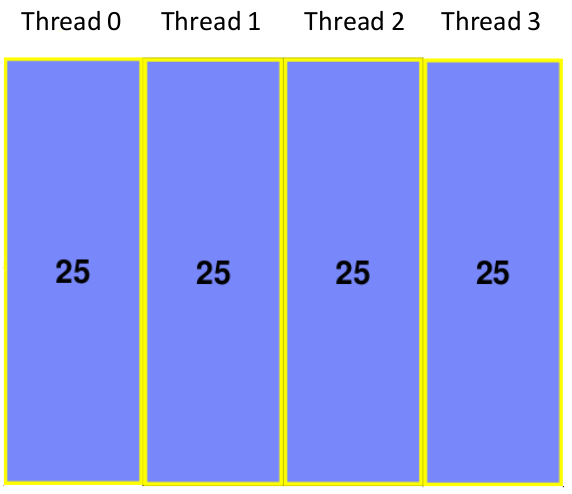
\includegraphics[width=.5\linewidth]{wiki/static_scheduling.png}
			\caption{Static Scheduling}
			\label{fig:sub1}
		\end{subfigure}
		\begin{subfigure}{.4\textwidth}
			\centering
			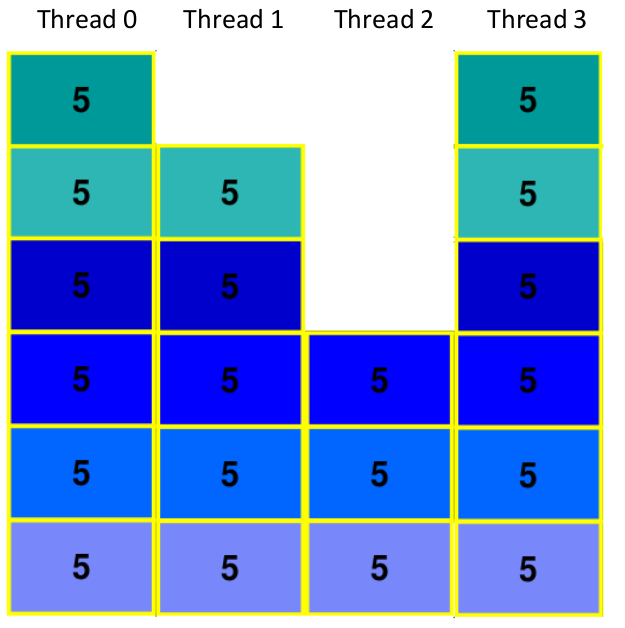
\includegraphics[width=.5\linewidth]{wiki/dynamic_scheduling.png}
			\caption{Dynamic Scheduling}
			\label{fig:sub2}
		\end{subfigure}
		\begin{subfigure}{.4\textwidth}
			\centering
			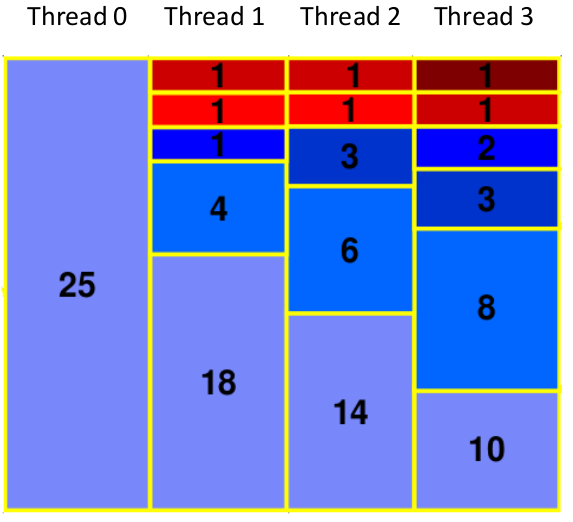
\includegraphics[width=.5\linewidth]{wiki/guided_scheduling.png}
			\caption{Guided Scheduling}
			\label{fig:sub2}
		\end{subfigure}
		\caption{Different Scheduling Strategies for 100 Iterations and 4 Threads}
		\label{fig:Scheduling}
	\end{figure}

	
	
\end{frame} 

\begin{frame}{OpenMP Scheduling - Results MP-Media}
\note{
	\begin{itemize}
		\item Static and Guided perform best
		\item Expected due to overhead
	\end{itemize}
}
	\centering
	\vspace{-5pt}
	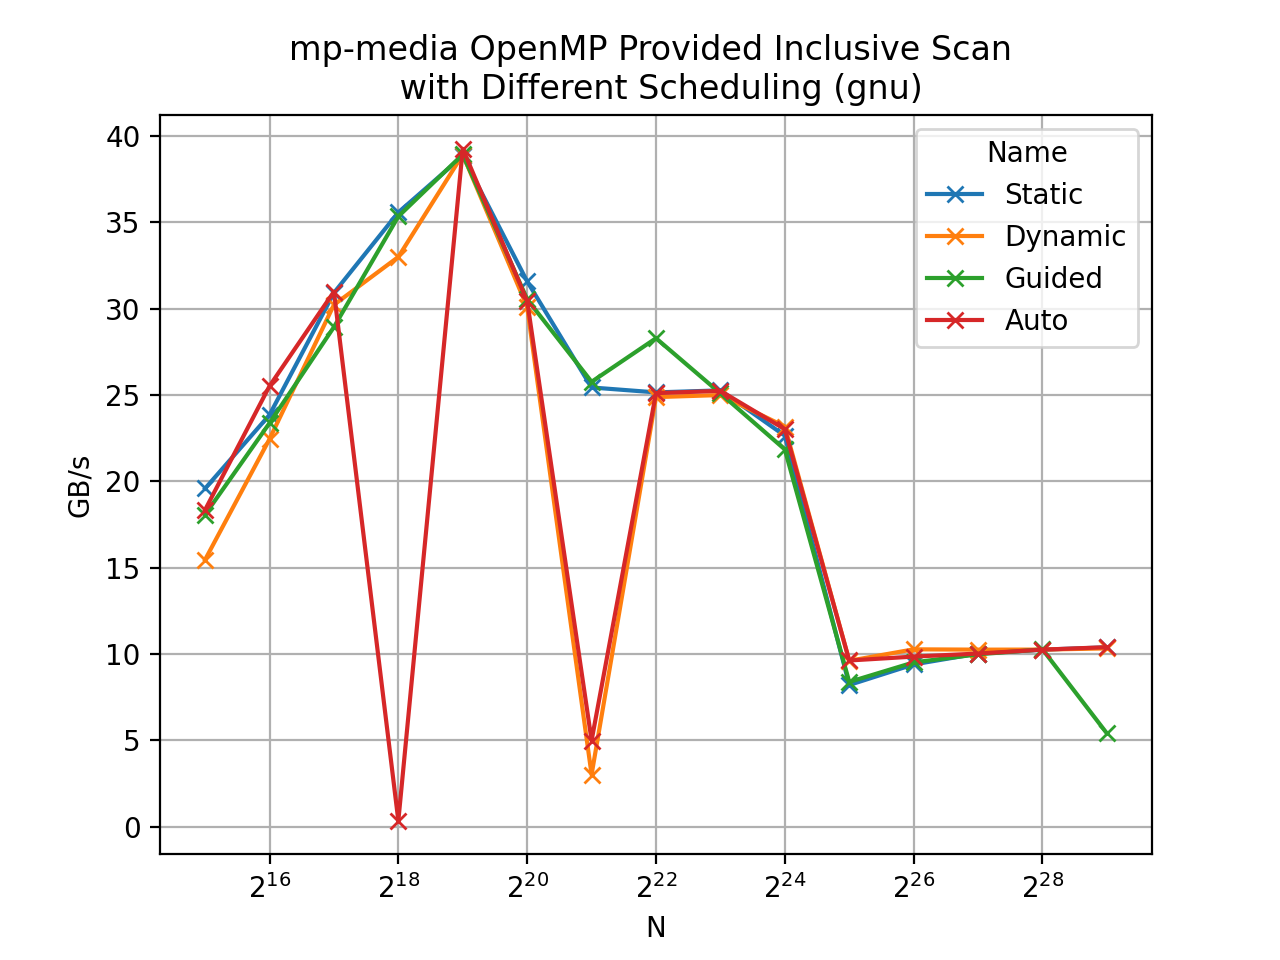
\includegraphics[width=0.90\textwidth]{graphs/mp-media OpenMP Provided Inclusive Scan  with Different Scheduling (gnu).png}
\end{frame}

\begin{frame}{OpenMP Scheduling - Results Ziti-Rome}
\note{
	\begin{itemize}
		\item More severe difference
		\item Static least overhead
		\item Static Bound size and Distribution of Work
		\item => Static best
	\end{itemize}
}
	\centering
	\vspace{-5pt}
	\includegraphics[width=0.90\textwidth]{graphs/ziti-rome OpenMP Provided Inclusive Scan  with Different Scheduling (gnu).png}
\end{frame}
